\documentclass[tikz,border=2pt]{standalone}
\usepackage{tikz}
\usetikzlibrary{arrows.meta,positioning,calc}
\renewcommand{\familydefault}{\sfdefault}
\begin{document}
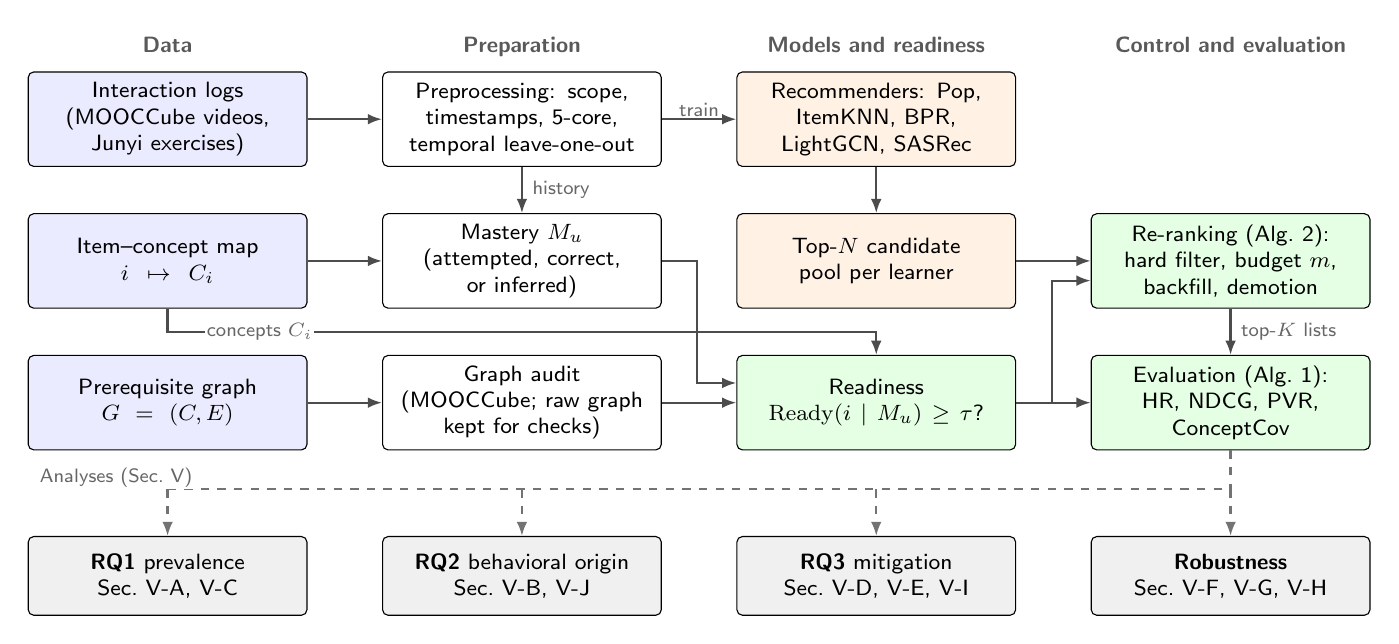
\begin{tikzpicture}[
  font=\sffamily\footnotesize, x=1mm, y=1mm,
  box/.style={draw, rounded corners=2pt, align=center, minimum height=12mm, text width=33mm, inner sep=1.2mm, fill=#1},
  box/.default=white,
  abox/.style={draw, rounded corners=2pt, align=center, minimum height=10mm, text width=33mm, inner sep=1.2mm, fill=gray!12},
  arr/.style={-{Latex[length=1.8mm]}, thick, draw=black!70},
  lab/.style={font=\sffamily\scriptsize, text=black!60, fill=white, inner sep=0.6pt},
  stage/.style={font=\sffamily\bfseries\footnotesize, text=black!65}]
% column x positions and row y positions (mm)
\def\xa{0}\def\xb{45}\def\xc{90}\def\xd{135}
\def\ya{0}\def\yb{-18}\def\yc{-36}
% ---- column 1: data ----
\node[box=blue!8] (logs)  at (\xa,\ya) {Interaction logs\\(MOOCCube videos,\\Junyi exercises)};
\node[box=blue!8] (map)   at (\xa,\yb) {Item--concept map\\$i \mapsto C_i$};
\node[box=blue!8] (graph) at (\xa,\yc) {Prerequisite graph\\$G=(C,E)$};
% ---- column 2: preparation ----
\node[box] (prep)    at (\xb,\ya) {Preprocessing: scope,\\timestamps, 5-core,\\temporal leave-one-out};
\node[box] (mastery) at (\xb,\yb) {Mastery $M_u$\\(attempted, correct,\\or inferred)};
\node[box] (audit)   at (\xb,\yc) {Graph audit\\(MOOCCube; raw graph\\kept for checks)};
% ---- column 3: models and readiness ----
\node[box=orange!10] (rec)   at (\xc,\ya) {Recommenders: Pop,\\ItemKNN, BPR,\\LightGCN, SASRec};
\node[box=orange!10] (pool)  at (\xc,\yb) {Top-$N$ candidate\\pool per learner};
\node[box=green!10]  (ready) at (\xc,\yc) {Readiness\\$\mathrm{Ready}(i\mid M_u)\geq\tau$?};
% ---- column 4: control and evaluation ----
\node[box=green!10] (rerank) at (\xd,\yb) {Re-ranking (Alg.~2):\\hard filter, budget $m$,\\backfill, demotion};
\node[box=green!10] (eval)   at (\xd,\yc) {Evaluation (Alg.~1):\\HR, NDCG, PVR,\\ConceptCov};
% ---- arrows ----
\draw[arr] (logs) -- (prep);
\draw[arr] (map) -- (mastery);
\draw[arr] (graph) -- (audit);
\draw[arr] (prep) -- node[lab, right=1mm] {history} (mastery);
\draw[arr] (prep) -- node[lab, above] {train} (rec);
\draw[arr] (rec) -- (pool);
\draw[arr] (pool) -- (rerank);
\draw[arr] (audit) -- (ready);
% the item--concept map is also needed for Req(i) of each candidate
\draw[arr] (map.south) -- (\xa,-27) -- node[lab, pos=0.13] {concepts $C_i$} (\xc,-27) -- (ready.north);
\draw[arr] (mastery.east) -- ++(4.5,0) |- ([yshift=2.5mm]ready.west);
\draw[arr] (ready.east) -- ++(4.5,0) |- ([yshift=-2.5mm]rerank.west);
\draw[arr] (ready) -- (eval);
\draw[arr] (rerank) -- node[lab, right=1mm] {top-$K$ lists} (eval);
% ---- analyses row ----
\def\ye{-58}
\node[abox] (rq1) at (\xa,\ye) {\textbf{RQ1} prevalence\\Sec.~V-A, V-C};
\node[abox] (rq2) at (\xb,\ye) {\textbf{RQ2} behavioral origin\\Sec.~V-B, V-J};
\node[abox] (rq3) at (\xc,\ye) {\textbf{RQ3} mitigation\\Sec.~V-D, V-E, V-I};
\node[abox] (rob) at (\xd,\ye) {\textbf{Robustness}\\Sec.~V-F, V-G, V-H};
\draw[thick, dashed, draw=black!55] (eval.south) -- (\xd,-47);
\draw[thick, dashed, draw=black!55] (\xa,-47) -- (\xd,-47);
\foreach \n/\x in {rq1/\xa, rq2/\xb, rq3/\xc, rob/\xd} \draw[arr, dashed, draw=black!55] (\x,-47) -- (\n.north);
\node[lab, anchor=south west] at (\xa-16.5,-47) {Analyses (Sec.~V)};
% ---- stage labels (same baseline for all columns) ----
\foreach \x/\t in {\xa/Data, \xb/Preparation, \xc/Models and readiness, \xd/Control and evaluation}
  \node[stage, anchor=base] at (\x,8.5) {\t};
\end{tikzpicture}
\end{document}
